%%%%%%%%%%%%%%%%%%%%%%%%%%%%%%%%%%%%%%%%%
% Beamer Presentation
% LaTeX Template
% Version 1.0 (10/11/12)
%
% This template has been downloaded from:
% http://www.LaTeXTemplates.com
%
% License:
% CC BY-NC-SA 3.0 (http://creativecommons.org/licenses/by-nc-sa/3.0/)
%
%%%%%%%%%%%%%%%%%%%%%%%%%%%%%%%%%%%%%%%%%

%----------------------------------------------------------------------------------------
%	PACKAGES AND THEMES
%----------------------------------------------------------------------------------------

\documentclass{beamer}
\beamertemplatenavigationsymbolsempty
\usepackage{ragged2e}
\usepackage{etoolbox}
\usepackage{lipsum}

\setbeamertemplate{caption}[numbered]
\mode<presentation> {

% The Beamer class comes with a number of default slide themes
% which change the colors and layouts of slides. Below this is a list
% of all the themes, uncomment each in turn to see what they look like.

%\usetheme{default}
%\usetheme{AnnArbor}
%\usetheme{Antibes}
%\usetheme{Bergen}
%\usetheme{Berkeley}
%\usetheme{Berlin}
%\usetheme{Boadilla}
%\usetheme{CambridgeUS}
%\usetheme{Copenhagen}
%\usetheme{Darmstadt}
%\usetheme{Dresden}
%\usetheme{Frankfurt}
%\usetheme{Goettingen}
%\usetheme{Hannover}
%\usetheme{Ilmenau}
%\usetheme{JuanLesPins}
%\usetheme{Luebeck}
%\usetheme{Madrid}
%\usetheme{Malmoe}
\usetheme{Marburg}
%\usetheme{Montpellier}
%\usetheme{PaloAlto}
%\usetheme{Pittsburgh}
%\usetheme{Rochester}
%\usetheme{Singapore}
%\usetheme{Szeged}
%\usetheme{Warsaw}
%\usetheme{Hannover-rose}



% As well as themes, the Beamer class has a number of color themes
% for any slide theme. Uncomment each of these in turn to see how it
% changes the colors of your current slide theme.

%\usecolortheme{albatross}
%\usecolortheme{beaver}
%\usecolortheme{beetle}
%\usecolortheme{crane}
%\usecolortheme{dolphin}
%\usecolortheme{dove}
%\usecolortheme{fly}
%\usecolortheme{lily}
%\usecolortheme{orchid}
%\usecolortheme{rose}
%\usecolortheme{seagull}
%\usecolortheme{seahorse}
%\usecolortheme{whale}
%\usecolortheme{wolverine}

%\setbeamertemplate{footline} % To remove the footer line in all slides uncomment this line
%\setbeamertemplate{footline}[page number] % To replace the footer line in all slides with a simple slide count uncomment this line

%\setbeamertemplate{navigation symbols}{} % To remove the navigation symbols from the bottom of all slides uncomment this line
}


\usepackage{graphicx} % Allows including images
\usepackage{booktabs} % Allows the use of \toprule, \midrule and \bottomrule in tables

%----------------------------------------------------------------------------------------
%	TITLE PAGE
%----------------------------------------------------------------------------------------

\title{Leakage-Resilient Password Entry on
Head-Mounted Smart Wearable Glass Devices} % The short title appears at the bottom of every slide, the full title is only on the title page

\author{ABHIJITH K D \\S7 CS B } % Your name
\institute[College of Engineering Cherthala] % Your institution as it will appear on the bottom of every slide, may be shorthand to save space
{
\begin{small}
Guided By:\\ \vspace{0.5em}  Mrs.Anitha M A
\end{small}
\\Department of Computer Science and Engineering \\ % Your institution for the title page
\medskip
%\textit{john@smith.com} % Your email address
}
\date{$22^{nd}$ October 2020} % Date, can be changed to a custom date

\setbeamertemplate{footline}[frame number]
\addtobeamertemplate{footline}{\hskip-46em College of Engineering Cherthala}{}
\addtobeamertemplate{footline}{\hskip35em $22^{nd}$ October 2020 - Seminar}{}


\begin{document}

\begin{frame}
\titlepage % Print the title page as the first slide
\end{frame}

\begin{frame}
\frametitle{Overview} % Table of contents slide, comment this block out to remove it
\tableofcontents % Throughout your presentation, if you choose to use \section{} and \subsection{} commands, these will automatically be printed on this slide as an overview of your presentation
\end{frame}

%----------------------------------------------------------------------------------------
%	PRESENTATION SLIDES
%----------------------------------------------------------------------------------------


\section{INTRODUCTION}
\begin{frame}
\frametitle{INTRODUCTION}

\justifying

\begin{itemize}

\justifying

\item Head-mounted smart wearable glass devices[5] are becoming popular.\newline
e.g: Google Glass[3], HoloLens[4].

\item Services : Email, Social media, maps etc.

\item  Privacy of Google glasses is a concern.
\item  Better authentication methods are needed for better security..

\begin{figure}
    \begin{center}
        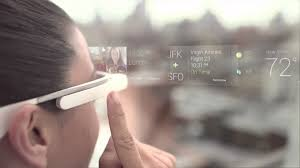
\includegraphics[scale=.55]{aplication.jpg}
        \caption{Smart Glass}
    \end{center}
\end{figure}


%\item Build a nanophotonic reservoir by exploiting and combining fast non linear light interactions to manipulate light
\end{itemize}
\end{frame}

\begin{frame}
\frametitle{INTRODUCTION (Contd.)}
\begin{figure}
    \begin{center}
        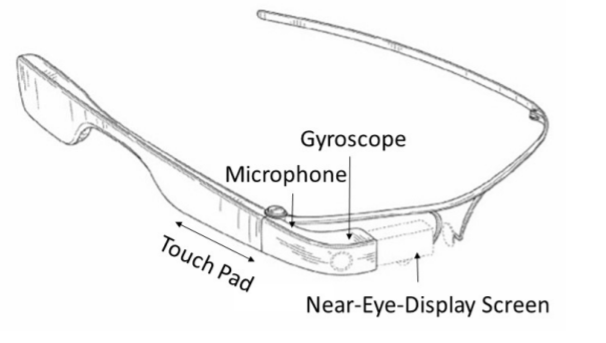
\includegraphics[scale=.35]{google.png}
        \caption{The Design of Google Glass}
    \end{center}
\end{figure}
\begin{itemize}

\justifying

\item 4 major parts : Touch Pad, NED Screen, Microphone, Gyroscope[6].
\item Rely on additional devices for password entry.
\item It will leads to a scope of \textbf{Eavesdropping attacks[7]:} 
\begin{enumerate}
\item External Eavesdropping attack
\begin{enumerate}
\item Vision-based attacks
\item Motion-based attacks
\item Acoustics-based attacks
\end{enumerate}
\item Internal Eavesdropping attack
\begin{enumerate}
\item Privileged attacks
\item Unprivileged attacks
\end{enumerate}
\end{enumerate}

%\item Build a nanophotonic reservoir by exploiting and combining fast non linear light interactions to manipulate light
\end{itemize}
\end{frame}

\begin{frame}
\frametitle{ Problems Overview }
\begin{itemize}
\item The switching between multiple devices for password entry.
\item Password entry in outdoors or public area.
\item A password enrty scheme within the limited hardware.
\item A password entry scheme which cannot be traceable by eavesdropping attackers.
\end{itemize}
\end{frame}

\begin{frame}
\section{DESIGN OVERVIEW}
\frametitle{DESIGN OVERVIEW}


\begin{itemize}

\justifying

\item To ensure security for smart glasses, three anti-eavesdropping password entry schemes:
\begin{enumerate}
\item gTapper
\item gRotator
\item gTalker
\end{enumerate}
\begin{figure}
    \begin{center}
        
\includegraphics[scale=.35]{symbols.jpg}
    \end{center}
\end{figure}


\item  Our \textbf{Design goals} are :
\begin{itemize}
\item  No additional devices or external hardware to be
involved.
\item  No password information except password length might be leaked.
\end{itemize}


%\item Build a nanophotonic reservoir by exploiting and combining fast non linear light interactions to manipulate light
\end{itemize}
\end{frame}


\section{gTapper}
\begin{frame}
\frametitle{gTapper}

\begin{itemize}

\justifying

\item Designed based on the small touch-pad.

\item The pad accepts user's finger gestures as input signals.
\item  Tapping, Pressing, and Swiping.
\item  Forward \& Backward, Up \& Down.

\end{itemize}

\begin{figure}
    \begin{center}
        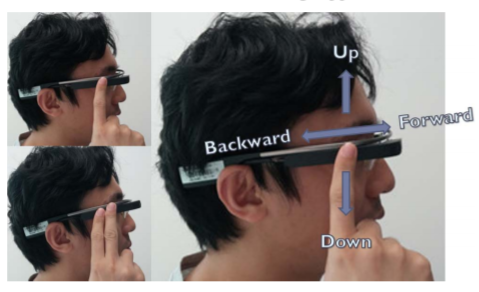
\includegraphics[scale=.55]{touchpad.png}
        \caption{Touch pad Gestures}
    \end{center}
\end{figure}

\end{frame}

\begin{frame}
\frametitle{gTapper}
\begin{figure}
    \begin{center}
        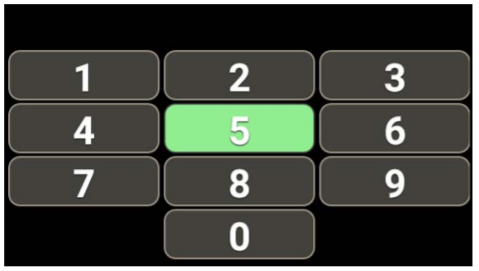
\includegraphics[scale=.50]{gTapper.png}
        \caption{Demonstration of gTapper}
    \end{center}
\end{figure}

\justifying

\begin{itemize}
\justifying

\item The Password alphabet $\Omega$ to be comprised of all single-digit numbers from 0 to 9.
\item In each round i, gTapper randomly
selects a number \newline $s_i$ $\epsilon$ \{ 0, 1, 2,..., 9 \} and sets the focus on that number.

\item Users can use one finger to shift the number focus to \newline ($s_i$ - 1) mod 10 or
($s_i$ + 1) mod 10, by swiping forward once or by swiping backward once.

\end{itemize}
\end{frame}
\justifying
\begin{frame}
\frametitle{gTapper}
\begin{itemize}
\justifying

\item To enter a password element $p_i$ $\epsilon$ {0, 1, 2,..., 9} in round
i, a user has to shift the number focus to $p_i$ on the keypad
from the initially focused number $s_i$ by swiping forward or
backward for $op_i$ times, where $op_i$ = ($s_i$ - $p_i$) mod 10 or
$op_i$ = ($p_i$ - $s_i$) mod 10 respectively. Then the user can enter
the selected number pi with a one-finger tap on the touch
pad.

\item \textbf{Security Analysis of gTapper :}
\begin{itemize}
\justifying
\item Attackers can know the number and the directions of shifts from the initially focused number to the $i^{th}$ element of the password.

\item But, the hidden keypad is protected
\item It is hard for attackers
to know the initially focused number.
\item Therefore cannot infer the $i^{th}$ element of the password.
\end{itemize}
\end{itemize}
\end{frame}

\section{gRotator}
\begin{frame}
\frametitle{gRotator}
\begin{itemize}

\justifying

    \item The design of gRotator relies on a gyroscope[6].
    \item The password alphabet $\Omega$ comprises of single-digit numbers from 0 to 9.
    
    \item The hidden keypad  is comprised of two number
screens:\newline
$C_s$ :Small number screen, $C_b$ :Big number screen.
    
 \begin{figure}
    \begin{center}
        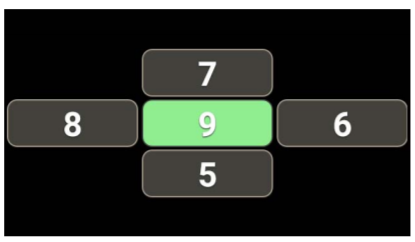
\includegraphics[scale=.50]{gRotator.PNG}
        \caption{Demonstration of gRotator}
    \end{center}
\end{figure}
    \item In each round i, five numbers and their positions
would be randomly shuffled.
    \item To change the number screen, users have to swipe
forward.
    
\end{itemize}
\end{frame}


\begin{frame}
\frametitle{gRotator (Contd.)}

\begin{figure}
    \begin{center}
        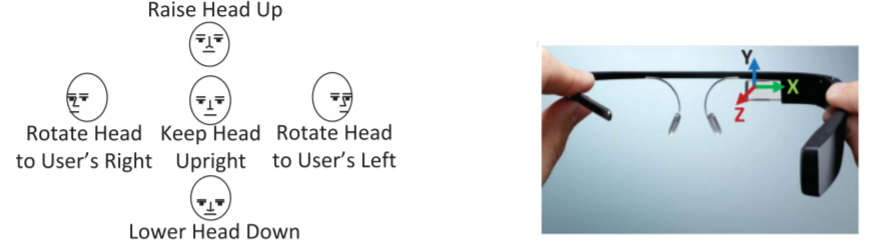
\includegraphics[scale=.45]{movements.png}
        \caption{Head movements in gRotator \& a typical motion sensor coordinate system on smart glasses.}
    \end{center}
\end{figure}


\justifying

\begin{itemize}

    \item Users may need to select a number by rotating head towards up, down, left or right.
   \item To track users’ head movements,
we use motion data captured by the gyroscope, including angular speeds on three orthogonal axes (ie. axis X, axis Y \& axis Z).
\end{itemize}

\end{frame}


\begin{frame}
\frametitle{gRotator (Contd.)}

\justifying

\begin{itemize}

\justifying

    \item  In terms of the angular speed, we can estimate
user's head rotation using a dead-reckoning algorithm[8].\newline Let
$R_{t_{i}}$ = ($r_{x,t_i}$,$r_{y,t_i}$,$r_{z,t_i}$) be the angular speed generated by the
gyroscope at time $t_i$.
    
    \item The rotation angle along each axis can be
calculated by the trapezoidal rule[9] for integral approximation
as follows.\newline
$\theta_{s,t_{i}}$ = ($r_{s,t_{i-1}}$ + $r_{s,t_{i}}$) · ($t_i$ - $t_{i-1}$)/2 \newline 
Where s $\epsilon$ \{x,y,z\}
    
    \item For simplicity, we use angle $\theta_{x,t_{i}}$ and angle $\theta_{y,t_{i}}$ to determine the up/down
directions and left/right directions of head movements.
    \item The initial head pose is calibrated and set at the
moment when a user initially launches gRotator.
\end{itemize}
\end{frame} 


\begin{frame}
\frametitle{gRotator (Contd.)}

\begin{itemize}

\justifying

    \item To avoid the inaccurate
control of head poses, we apply thresholds:\newline
$\xi_v$ : up/down,   $\xi_h$ : left/right
    
    \item  The estimation of head rotation direction
$H_{t_{i}}$ at time $t_i$ can be computed as below. 
\begin{figure}
    \begin{center}
        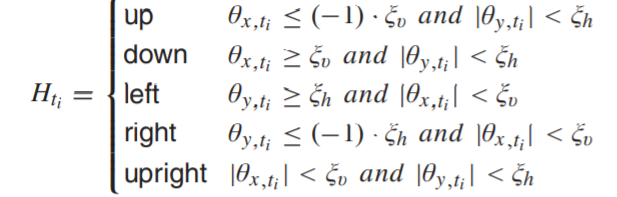
\includegraphics[scale=.50]{equation.png}
    \end{center}
\end{figure}
    
    \item \textbf{Security Analysis of gRotator:}
    \begin{itemize}
    \item  The keypad, including the two number screens is hidden.
    \item  In each round i, five numbers and their positions
would be randomly shuffled.

    \end{itemize}
\end{itemize}

\end{frame}

\section{gTalker}
\begin{frame}
\frametitle{gTalker}

\begin{itemize}
\justifying

%    \item Consider a Web of Things Scenario, which is a Connected Hotel.
    
    \item The design of gTalker depends on a speech
    recognition-enabled built-in microphone.
    
    \item  gTalker adopts the alphabet of password word as \newline $\Omega$= \{0, 1, 2,..., 9\}.
    
    \item Every white number p is followed by an underlined red number s.
    \item In each round i,\newline White numbers(p) :Constant positions\newline Red numbers(s): shuffle their
positions.
\end{itemize}

\begin{figure}
    \begin{center}
        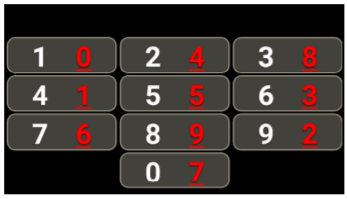
\includegraphics[scale=.50]{gTalker.png}
        \caption{Demonstration of gTalker.}
    \end{center}
\end{figure}

\end{frame}

\begin{frame}
\frametitle{gTalker (Contd.)}

\begin{itemize}
\justifying
    
    \item For each white number $p_k$ = k, let $s_{ik}$
denote the corresponding underlined red number in round i,
where k $\epsilon$ $\Omega$  and $s_{ik}$ $\epsilon$ $\Omega$. For 	\forall j, k $\epsilon$ $\Omega$  and j \neq k, \hspace{2}   $s_{ij}$\neq$s_{ik}$ 
holds.
    
    \item  To enter password element k, users have to
firstly identify the position of  $p_k$, and then
speak out the underlined red number $s_{ik}$.
    
    \item The mapping between $p_k$ \& $s_{ik}$ identify the password element k.
    \item gTalker uses an offline speech
recognition function available in Android API[10], which is
developed based on Deep Neural Networks with Hidden Markov
Models (DNN-HMM)[11]
\item \textbf{Security Analysis of gTalker:}
\begin{itemize}
    \item The adversary does not know the random mapping
between the original keypad and the transformed keypad.
\end{itemize}

\end{itemize}


\end{frame}

\section{DATA COLLECTION \& EVALUATION}
\begin{frame}
\frametitle{DATA COLLECTION \& EVALUATION}

\begin{itemize}
\justifying
    
    \item 3 schemes- IRB[12] approved user study:
    
    \item  \textbf{Normal condition:}  No time limit, Fixed number of attempt.
    \item \textbf{Timed Condition:} Time limit, Any no.of attempt.
    \item \textbf{No distraction.}
    \item \textbf{Distraction[13].}
    \item \textbf{Heavy distraction[13].}
    \item \textbf{Average Login Time \& Login Success Rate.}
\end{itemize}


\end{frame}

\begin{frame}
\frametitle{Results Analysis}

\begin{itemize}
\justifying
    
    \item \textbf{Normal Condition.}
    \begin{figure}
    \begin{center}
        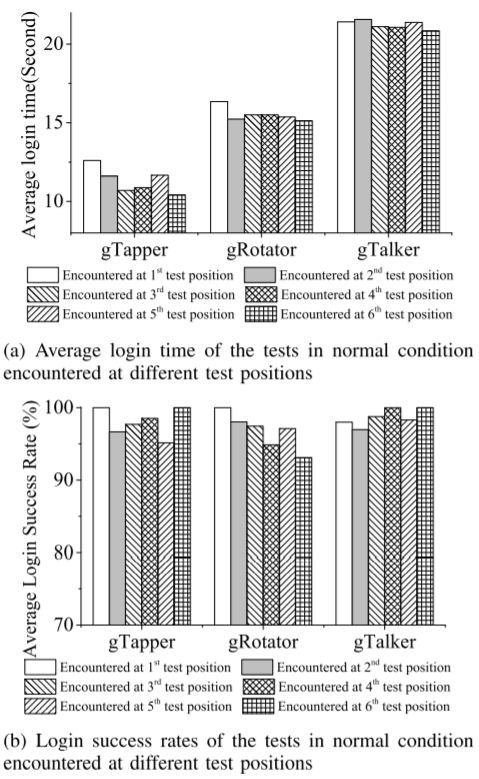
\includegraphics[scale=.33]{test1.png}
        \caption{Learning curves for gTapper, gRotator, and gTalker}
    \end{center}
\end{figure}    


    \item Login time decreases as test position increases.
    \item Change in the test positions would not affect the login success rate.

\end{itemize}


\end{frame}

\begin{frame}
\frametitle{Results Analysis}

\begin{itemize}
\justifying
    
    \item \textbf{Normal Condition Vs Timed Condition.}
    \begin{figure}
    \begin{center}
        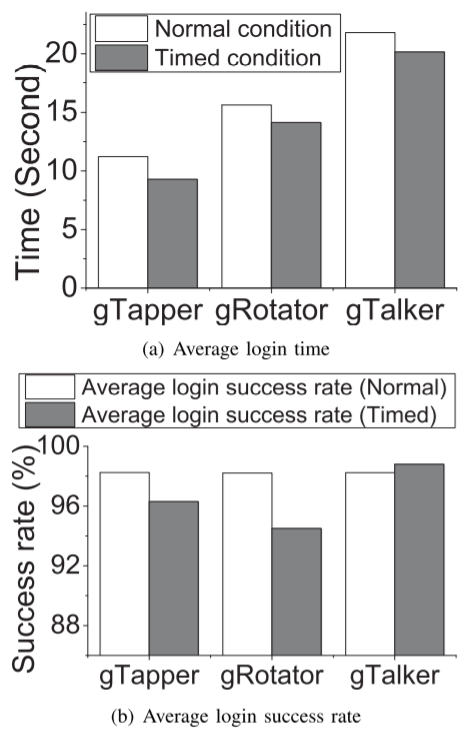
\includegraphics[scale=.33]{test2.png}
        \caption{Impact of time pressure}
    \end{center}
\end{figure}    


    \item Login time decreases in Timed condition.
    \item Timed condition doesn't effect the success rate due to ceiling effect[14].

\end{itemize}


\end{frame}

\begin{frame}
\frametitle{Results Analysis}

\begin{itemize}
\justifying
    
    \item \textbf{Impact of Distraction.}
    \begin{figure}
    \begin{center}
        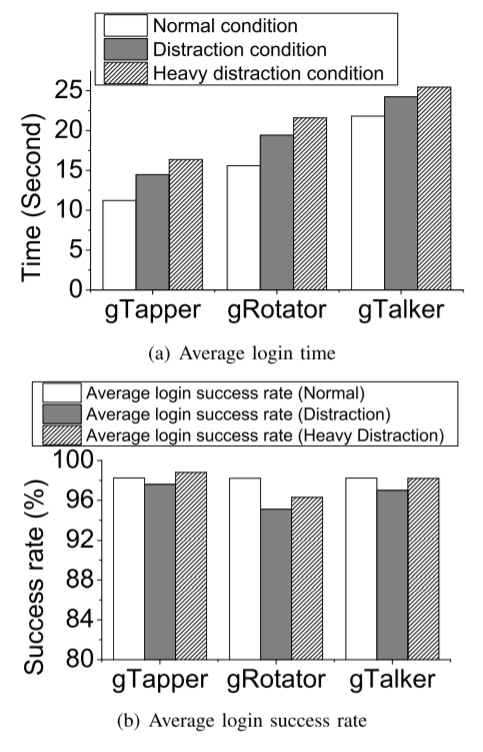
\includegraphics[scale=.33]{test3.png}
        \caption{Impact of distraction}
    \end{center}
\end{figure}    


    \item Login time increases with Distractions.
    \item Distractions doesn't effect the success rate.

\end{itemize}


\end{frame}

\begin{frame}
\frametitle{Evaluation Results Overview}

\begin{itemize}
\justifying
    
    \item Login time decreases as test position increases.
    \item Login time decreases under timed condition.
    \item Login time increases with Distractions.
    \item Login success rate is not effected by test positions, time pressure, distractions.

\end{itemize}


\end{frame}

\section{COMPARISONS}
\begin{frame}
\frametitle{COMPARISONS}

\begin{itemize}
\justifying
    
    \item \textbf{gTaper Vs gRotator Vs gTalker.}
    
    \begin{figure}
    \begin{center}
        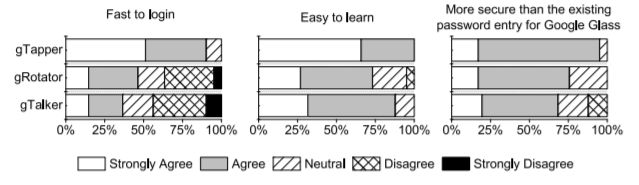
\includegraphics[scale=.65]{comp1.png}
        \caption{Comparison of 3 schemes}
    \end{center}
\end{figure}
    
    \item \textbf{gTaper:} Very easy to learn, Very fast login, Secure.
    \item \textbf{gRotator:} Easy to learn, Slow login than gTaper, Secure.
    \item \textbf{gTalker:} Easy to learn, Slow login than gRotator, Secure.

\end{itemize}


\end{frame}

\begin{frame}
\frametitle{COMPARISONS}

\begin{itemize}
\justifying
    
    \item \textbf{Proposed scheme Vs Existing schemes.}
    
    \begin{figure}
    \begin{center}
        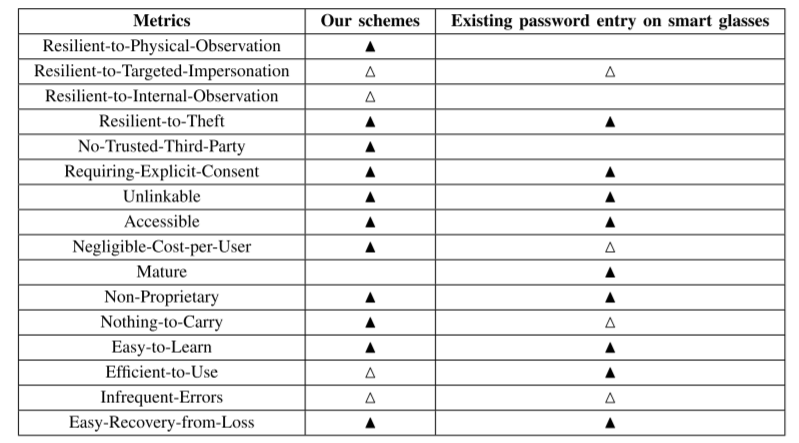
\includegraphics[scale=.50]{comp2.png}
        \caption{Comparison of 3 schemes}
    \end{center}
\end{figure}
    
    \item \textbf{Dark Triangle:} Benefit is offered.
    \item \textbf{Bright Triangle:} Benefit is partially offered.
    \item \textbf{Blank Cell:} Benefit is not offered.

\end{itemize}


\end{frame}

\section{ADVANTAGES}
\begin{frame}
\frametitle{ ADVANTAGES }
\begin{itemize}
\item More secure than conventional password entry.
\item Can avoid switching between multiple devices.
\item Easy to use in outdoors.
\item Uses only the available hardware in smart glasses.
\end{itemize}
\end{frame}

\section{DISADVANTAGES}
\begin{frame}
\frametitle{ DISADVANTAGES }
\begin{itemize}
\item Don't have a richer password alphabet.
\item Password length is less.
\item Speech recognition[11].
\item Head movement estimation[1].
\item Sometimes password entry takes more time.
\end{itemize}
\end{frame}

\begin{frame}
\frametitle{ THINK ABOUT IT }

\textbf{\Large"Richer password alphabet only requires a shorter password length"}

\end{frame}

\section{SOLUTIONS}
\begin{frame}
\frametitle{ SOLUTIONS }
\begin{itemize}
\item More richer set of alphabet by using AR[15] \& VR[16].
\begin{figure}
    \begin{center}
        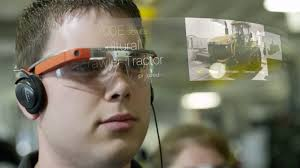
\includegraphics[scale=.60]{ar.jpg}
        \caption{Demonstration of AR-VR[15][16] in google glass.}
    \end{center}
\end{figure}
\item  Bio-metric[17] sensors like fingerprint recognition, iris recognition etc. for password entry.
\end{itemize}
\end{frame}

\section{CONCLUSION}
\begin{frame}
\frametitle{CONCLUSION}
\begin{itemize}
\justifying
\item At present, most existing anti-eavesdropping password entry
schemes on smart glasses are heavily depending on additional devices.
\item So users neeed to switch between different systems and devices.
\item Three anti-eavesdropping password
entry schemes for smart glasses: named gTapper, gRotator
and gTalker.
\item These 3 schemes provides better security for smart glasses from  the eavesdropping attacks.
\item Don't need to switch between devices.
\item These schemes Don't use any extra hardware.
\item An an IRB-approved users study conducted.
\item Out of 3 schemes, gTapper is easy to use and has a fast login.
and these 3 schemes provides more security than other schemes.
\item Designed schemes are easy to use in various real-world scenarios.
\end{itemize}
\end{frame}




%----------------------------------------------
\section{REFERENCES}
\begin{frame}[allowframebreaks]
\frametitle{REFERENCES}
\begin{enumerate}
\tiny


\bibitem{a}{ Yan Li, Y. Cheng,Weizhi Meng, Yingjiu Li and R. H. Deng \textquotedblleft Designing Leakage-Resilient Password Entry on
Head-Mounted Smart Wearable Glass Devices", \textit{ IEEE TRANSACTIONS ON INFORMATION FORENSICS AND SECURITY}, Volume: 16, Issue: 5, July 2020.  }

\bibitem{b}{Y. Li, Y. Cheng, Y. Li, and R. H. Deng \textquotedblleft “What you see is not
what you get: Leakage-resilient password entry schemes for smart
glasses,” \textit{ Computer Community}, in Proc. ACM Asia Conf. Comput. Commun. Secur., April 2017,
pp. 327–333  }

\bibitem{c} 	 {{\textquotedblleft Google. (2017). Google Glass\textquotedblright}. [Online]. Available:\\ \textit{https://developers.google.com/glass/distribute/glass-at-work} Accessed on: Sept. 28, 2020}

\bibitem{d} {\textquotedblleft  Microsoft. (2017). Microsoft Hololens \textquotedblright . [Online]. Available:\\ \textit{https://www.microsoft.com/microsoft-hololens/en-us} Accessed on: Sept. 28, 2020}

\bibitem{e} 	 {{\textquotedblleft Smart Wearable Devices \textquotedblright}. [Online]. Available:\\ \textit{https://www.gadgetsnow.com/slideshows/8-smart-wearables-you-must-know-about/photolist/51256562.cms} Accessed on: Oct. 12,2020}

\bibitem{f} 	 {{\textquotedblleft Wikipedia. Gyroscope \textquotedblright}. [Online]. Available:\\ \textit{https://en.wikipedia.org/wiki/Gyroscope} Accessed on: Oct. 12, 2020}

\bibitem{g} 	 {{\textquotedblleft Eavesdropping attack \textquotedblright}. [Online]. Available:\\ \textit{https://www.sciencedirect.com/topics/computer-science/eavesdropping-attack} \newline Accessed on: Oct. 12, 2020}

\bibitem{h} 	 {{\textquotedblleft Wikipedia. Dead Reckoning Algorithm \textquotedblright}. [Online]. Available:\\ \textit{https://en.wikipedia.org/wiki/Dead\_reckoning}  Accessed  on: Oct. 12, 2020}

\bibitem{i} 	 {{\textquotedblleft Wikipedia. Trapezoidal Rule \textquotedblright}. [Online]. Available:\\ \textit{https://en.wikipedia.org/wiki/Trapezoidal\_rule}   Accessed  on: Oct. 12, 2020}

\bibitem{j} 	 {{\textquotedblleft Wikipedia. API \textquotedblright}. [Online]. Available:\\ \textit{https://en.wikipedia.org/wiki/API}    Accessed  on: Oct. 12, 2020}




\bibitem{k} 	 {{\textquotedblleft Wikipedia. DNN-HMM \textquotedblright}. [Online]. Available:\\ \textit{https://en.wikipedia.org/wiki/Speech\_recognition} Accessed on: Oct. 12, 2020}

\bibitem{l} 	 {{\textquotedblleft Wikepedia. IRB \textquotedblright}. [Online]. Available:\\ \textit{https://en.wikipedia.org/wiki/IRB\_Infrastructure} Accessed on: Oct. 12, 2020}

\bibitem{m}{P. D. Adamczyk and B. P. Bailey \textquotedblleft If not now, when?: The effects of interruption at different moments within task execution,” \textit{ NDSS}, in Proc. Conf. Hum. Factors Comput. Syst., 2004, pp. 271–278}

\bibitem{n} 	 {{\textquotedblleft Wikepedia. Ceiling effect \textquotedblright}. [Online]. Available:\\ \textit{https://en.wikipedia.org/wiki/Ceiling\_effect\_(statistics)}   Accessed on: Oct. 12, 2020}

\bibitem{o} 	 {{\textquotedblleft Augmented Reality \textquotedblright}. [Online]. Available:\\ \textit{https://en.wikipedia.org/wiki/Augmented\_reality}  Accessed on: Oct. 12, 2020}

\bibitem{p} 	 {{\textquotedblleft Virtual Reality \textquotedblright}. [Online]. Available:\\ \textit{https://en.wikipedia.org/wiki/Virtual\_reality}  Accessed on: Oct. 12, 2020}

\bibitem{q} 	 {{\textquotedblleft Wikepedia. Biometrics \textquotedblright}. [Online]. Available:\\ \textit{https://en.wikipedia.org/wiki/Biometrics} Accessed on: Oct. 12, 2020}

\bibitem{}r{Q. Yan, J. Han, Y. Li, J. Zhou, and R. H. Deng \textquotedblleft Designing leakage resilient password entry on touchscreen mobile devices,” \textit{ Computer Community}, in Proc. 8th ACM SIGSAC Symp. Inf., Comput. Commun. Secur., 2013, pp. 37–48  }



\end{enumerate}

\end{frame}





%------------------------------------------------

\section*{THANK YOU}
\begin{frame}
\Huge{\centerline{\textbf{THANK YOU}}}
\end{frame}

%----------------------------------------------------------------------------------------

\end{document} 